\section{Parallel NOAH supersequences}
\label{sec:noah__parallel}

To conclude this chapter, I discuss how \textit{multiple} NOAH supersequences may be run in parallel in order to obtain yet more data from a single experiment.
As of the time of writing, current software limitations in TopSpin limit the \texttt{NBL} parameter (the number of memory blocks) to 5.
This makes it presently impossible to extend a supersequence linearly beyond five modules.
However, it is possible to \textit{interleave} different supersequences, such that one $t_1$ increment of supersequence A is acquired, followed by one $t_1$ increment of supersequence B, before the value of $t_1$ is increased for both supersequences.
In this text, I refer to this as a `vertical' stacking of modules (as opposed to the traditional NOAH concept, which focuses on `horizontal' concatenation of modules).

\begin{figure}[!htbp]
    \centering
    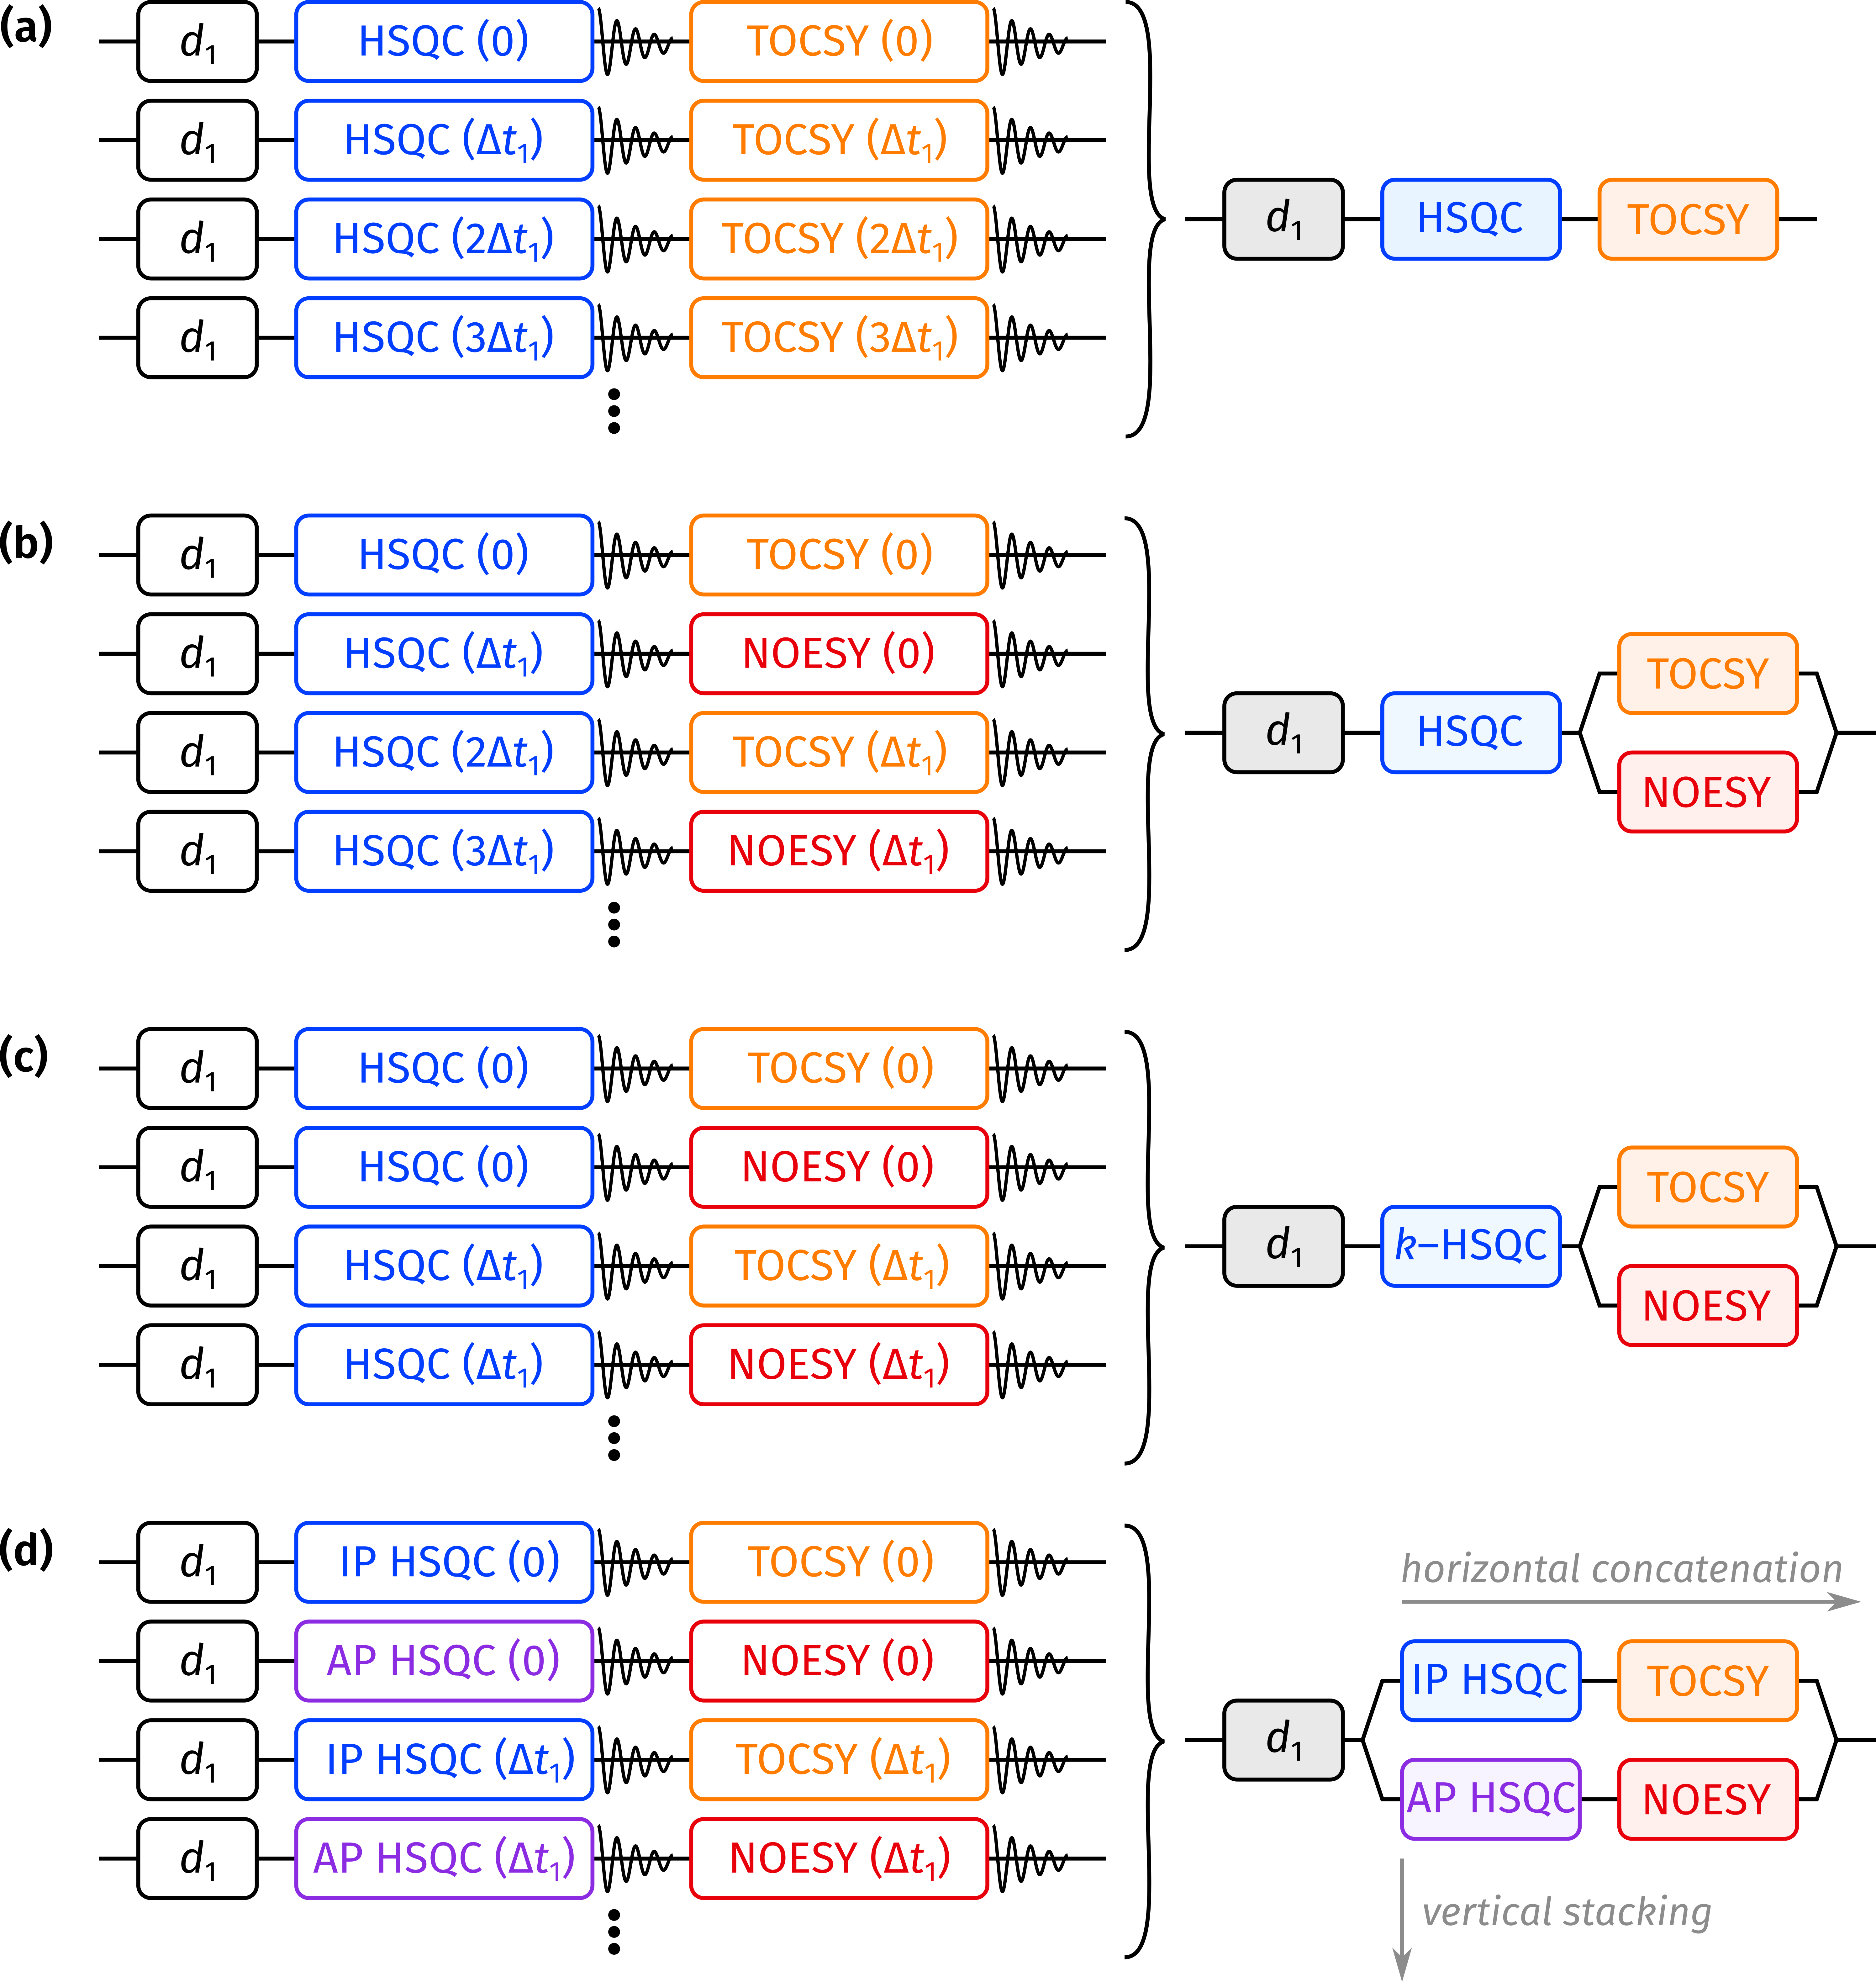
\includegraphics[draft=false]{noah/parallel_noah_overview.png}%
    {\phantomsubcaption\label{fig:parallel_noah_overview_conv}}%
    {\phantomsubcaption\label{fig:parallel_noah_overview_interleaved}}%
    {\phantomsubcaption\label{fig:parallel_noah_overview_kscaled}}%
    {\phantomsubcaption\label{fig:parallel_noah_overview_parallel}}%
    \caption[Overview of parallel NOAH supersequences]{
        An overview of `parallel' NOAH supersequences.
        The left side of each diagram explicitly spells out how $t_1$ is incremented for each module: the value in parentheses indicates the current value of $t_1$, which begins at 0 and is incremented by $\Delta t_1$ each time.
        The right side is a `condensed' depiction of the entire supersequence.
        \textbf{(\subref*{fig:parallel_noah_overview_conv})} A `standard' NOAH supersequence, where $t_1$ for every module is incremented at the same time.
        \textbf{(\subref*{fig:parallel_noah_overview_interleaved})} The first example of a `parallel' supersequence: the HSQC module is acquired as normal, but the TOCSY and NOESY modules are interleaved in the second slot.
        \textbf{(\subref*{fig:parallel_noah_overview_kscaled})} The same as in (\subref*{fig:parallel_noah_overview_interleaved}), but the HSQC module is subjected to $k$-scaling (see also \cref{subsec:noah__hmqc}).
        \textbf{(\subref*{fig:parallel_noah_overview_parallel})} A fully parallel supersequence, where both the first and second module slots are varied systematically.
        This amounts to the interleaved acquisition of two different `standard' supersequences.
    }
    \label{fig:parallel_noah_overview}
\end{figure}

This concept is more clearly illustrated in \cref{fig:parallel_noah_overview}, which contains a more explicit depiction of how $t_1$ is incremented for each module.
In \cref{fig:parallel_noah_overview_conv}, a `traditional' \noah{S,T} supersequence is shown: here, $t_1$ is incremented for both the HSQC and TOCSY module at the same time, and on each $t_1$ increment, the sequence of modules being acquired is always the same.
In \cref{fig:parallel_noah_overview_interleaved}, this is different: the second module is alternated between a TOCSY and a NOESY.
If the total experimental duration (which is largely proportional to the number of recovery delays, $d_1$) is to be kept the same as before, this means that the TOCSY and NOESY modules will be recorded with half the number of $t_1$ increments each.%
\footnote{The data must also be separated prior to Fourier transformation in the indirect dimension. This is `just' an implementation detail, but \textit{did} require the \texttt{splitx\_au} script to be substantially reworked.}
Although this loss of resolution may be considered a drawback, this scheme does allow us greater \textit{flexibility} in the design of NOAH supersequences: it is not ideal to acquire both a TOCSY and a NOESY using a traditional `linear' supersequence, since both of these modules depend on \magnnot{C} magnetisation.

\Cref{fig:parallel_noah_overview_kscaled} shows how the different $F_1$ resolutions can be `fixed' by performing the equivalent of $k$-scaling on the HSQC module (described in \cref{subsec:noah__hmqc}).
This entails reducing the number of $t_1$ increments by a factor of 2 (in this case), and acquiring each increment twice instead, which corresponds to a doubling of the number of scans after the data have been appropriately combined.
This generally has very little impact on the spectra (as was previously shown), but provides a convenient lead into the final example of \cref{fig:parallel_noah_overview_parallel}.
Here, instead of acquiring each increment of the HSQC module twice, the time is used to acquire two different modules, an in-phase (IP) and antiphase (AP) HSQC (both run without \carbon{} decoupling).
Through appropriate linear combination of the data, it is possible to isolate the two peaks of the \proton{}--\carbon{} doublets in these spectra, and from thence measure $\oneJ{CH}$ values: this is known as in-phase/antiphase (IPAP) processing.\autocite{Ottiger1998JMR,Nolis2006JMR,Enthart2008JMR,Gil2010JMR}
Much like the TOCSY and NOESY combination, it is not possible to acquire IP and AP HSQC spectra in a single, linear supersequence, not even with the partial \magn{C} excitation technique described in \cref{subsec:noah__hsqctocsy}.
For the IPAP processing to work, the IP and AP spectra have to be acquired with the same intensity for all peaks: even with a careful choice of $f$ in a linear supersequence, it is not possible to ensure this.

The reader will no doubt notice at this point that \cref{fig:parallel_noah_overview_parallel} corresponds simply to the interleaved acquisition of two different supersequences (one is IP-HSQC + COSY, and the other AP-HSQC + NOESY), which could just as well be acquired separately.
Furthermore, both supersequences are acquired with only half the usual $F_1$ resolution (assuming the same experimental time as \cref{fig:parallel_noah_overview_conv}), meaning that there are \textit{no real time savings}.
This is indeed correct: fundamentally, `vertical' stacking does not increase the number of FIDs recorded per recovery delay, so does not improve the time efficiency (or $\rho_t$).
The main benefits of this process are, in my opinion:
\begin{itemize}
    \item the \textit{flexibility} to construct supersequences that combine previously incompatible modules (such as in the examples above); and
    \item a way of \textit{adjusting for relative sensitivities of different modules}.
        For example, the arrangement in \cref{fig:parallel_noah_overview_kscaled} amounts to the acquisition of the HSQC module for $2n$ scans, and the TOCSY and NOESY modules for $n$ scans each (where $n$ is some positive integer).
        In this way, less intrinsically sensitive modules can be assigned a larger number of scans, such that all modules in the supersequence have (relatively) equalised intensities.
\end{itemize}

In principle, all of the above may still be accomplished by acquiring multiple separate supersequences and then combining the results appropriately.
However, the current implementation of parallel supersequences provides \textit{convenience} for the user, as all experiments may be simultaneously acquired and processed.
This factor should not be overlooked, especially considering that all the different constructions (\cref{fig:parallel_noah_overview_interleaved,fig:parallel_noah_overview_kscaled,fig:parallel_noah_overview_parallel}) must be processed in a slightly different manner: it is easier to do this from within a single experiment, rather than attempting to combine FIDs from separate datasets after the fact.


\todo{TS vs IPAP argument}

\todo{one example}


\subsection{Generalised supersequences}

\todo{Explain how these differ from parallel---different number of `threads' per module}

\todo{Balance sensitivities of modules}

\todo{Pulse sequence implementation}

\todo{Examples of such supersequences -- ADEQUATE/NHMBC stuff}

\todo{Covariance stuff in recent paper draft}
